\thispagestyle{plain}
\chapter{Framework}
This chapter introduces the framework that was implemented to generate workloads, partition data and eventually benchmark a custom index that uses the partitioning. Note that the terms partitions and segments will be used interchangeably in the following.
\begin{figure}[H]
    \centering
    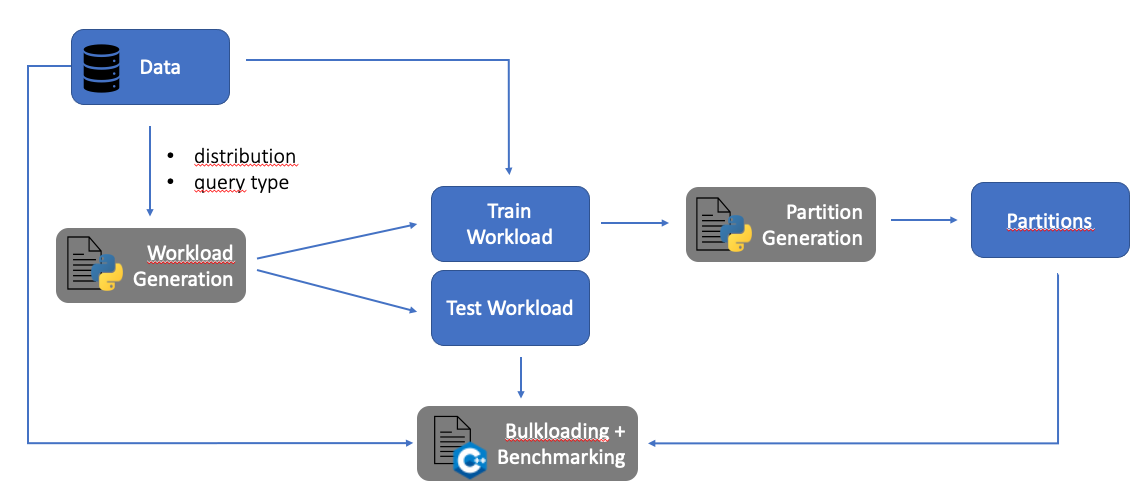
\includegraphics[width=\textwidth]{figures/pipeline.png}
    \caption{Framework Overview}
    \label{fig:framework}
\end{figure}

\section{Overview}
As we can see in Figure \ref{fig:framework}, the origin of all processes is the underlying data that should be indexed. Using a python script, we can specify properties like the distribution and type of queries (point, range) that should be generated to access the data through the index. The queries generated by this step are divided into a train and test workload and saved to files for later use in the C++ benchmarking.

TODO: Example of overlapping distributions

Given the train workload, the partitioning algorithms that are described in Sections \ref{sec:frequency} and \ref{sec:purity} can analyze the corresponding properties of the workload and will produce a partition of the underlying data. The resulting elements are saved to a file with additional information that can be used for the index construction.
With this partition, the index is bulkloaded from the data where each element of the partition corresponds to an individual leaf node. The additional information like relative frequency and predominant query type of a segment can be used to modify the index. For example, if only point queries access a segment, it could be beneficial to manage data access through a hash table instead of a normal B-tree leaf. The next step is to execute the test workload on the index and compare it to other state-of-the-art indexes that were introduced in Section \ref{sec:related_work}, namely a B$^+$-tree, an Adaptive Radix Tree (ART) and a Piecewise Geometric Model index (PGM).

\section{Workload Generation}
The ultimate goal of this work is to generate good partitions for the index construction like it was mentioned in Section \ref{bg:hybrid}. The inputs to the partitioning algorithms are therefore a dataset and a workload sample which we know is representative of the expected workload. However, for the purpose of evaluating and testing the algorithms and modifications later used, we were in need of a flexible way to generate workload data, especially since it proved hard to find available real-world workload data. The workload generation is done in a Python script specifying a series of \verb|Region| objects that wrap the following information:

\begin{itemize}
    \item \verb|qtype|: The query type that should be generated in this section, e.g.~point or range queries
    \item \verb|num|: The number of queries for this section
    \item \verb|distribution|: Distribution underlying the generated queries, e.g.~normal, uniform, ...
    \item \verb|index|: Whether the generation happens index-based or domain-based
    \item \verb|min, max|: minimal and maximal values that indicate the section boundaries. Either index or domain-based, depending on the value of \verb|index|.
\end{itemize}

This gives us a very flexible way to generate arbitrary workloads. Note that while a partition generated for the index construction later satisfies that the elements are mutually disjoint, the \verb|Region| objects used for workload generation do not need to be disjoint. This only means that we can overlap the boundaries of the objects to generate even more flexible workloads. In fact, it is the only way to generate regions of the data that are accessed through multiple types of queries, e.g.~ through both point and range queries. 

\section{Partitioning algorithms}
There are a plethora of properties that one could look at when analyzing query workloads, but inspired by the works in Section \ref{sec:related_work}, we decided to focus on two properties and look at how we could use these to partition the data and create segments. As described in the previous Section, we can use the train workload to partition the data. The test workload is immediately saved to file after creation and not seen by both partitioning algorithms. 

\subsection{Partitioning by Frequency} \label{sec:frequency}
The first algorithm analyzes the frequency of query access for each key in the key space. The motivation behind using the frequency as partition property is that hopefully we can benefit from caching effects during execution of the test workload. We would hope that highly frequent segments remain in cache so that subsequent queries can retrieve the location of the corresponding keys faster. Additionally, by analyzing the frequency, we can use that information to change the structure of the index. A first idea in this regard would be to shift highly frequent segments higher up in the tree, to prevent expensive pointer chasing when traversing the index.

We first realized, that key-by-key comparisons are not useful for a generalized partitioning algorithm because we can only operate on a train workload that is sampled from the general workload distribution. If we would use these key-by-key comparisons for the frequency to create partitions, we would probably overfit to the patterns in the train workload, even though these might only be caused by noise and not be present in the general distribution. Therefore, we employ an approach that tries to maximize the previously mentioned goal: find partitions where keys are accessed roughly the same amount of times. This partition should create elements, that utilize caching. Regions with almost no accesses will be put in one partition which will result in the segment being not loaded very often. On the other hand, regions with similarly frequent keys will result in the the corresponding segment remaining in cache if the frequency is high enough.

We use a single-pass algorithm that tries to find plateaus in the workload distribution by calculating the average change in frequency over a sliding window. It uses three phases depending on where it currently is with respect to a plateau, which are heavily inspired by the finite difference approximations from Section \ref{bg:numerical}:

\begin{enumerate}
    \item Start calculating a discrete forward difference approximation. As only keys "in the future" are considered, this phase is predestined to find an incoming plateau by checking if the calculated slope is near 0.
    \item After such a plateau was found, we use the central difference approximation to establish the boundaries of the plateau. We use this approximation now, as it considers keys from before and after the current one. This should give a better estimation of when a plateau is ending.
    \item Once the central approximation indicates that a plateau is ending, we switch to calculating the backward finite difference approximation to ensure that we find the exact end point of the plateau. We only consider previous keys, as we now know that an end is coming and this gives us the best chance to catch the key that is responsible for significantly changing the slope.
\end{enumerate}



\begin{algorithm}
\caption{Partition by Frequency}
\begin{algorithmic} 
    \STATE $idx \leftarrow 0$
    \STATE $n \leftarrow data.size$
    \WHILE{$idx < n - w$}
    \STATE $current\_freq \leftarrow freq[idx]$
    \STATE $fwd\_mean \leftarrow mean(freq[idx : idx + w])$
    \STATE $fwd\_slope \leftarrow fwd\_mean / w$
    \IF{$isclose(fwd\_slope, 0, delta / w)$}
    \STATE $potential\_start \leftarrow idx$
    \STATE $idx \leftarrow idx + 1$
    \FOR{$i \text{ in } 1 .. w // 2$}
    \STATE $central\_left \leftarrow mean(freq[idx - i : idx + 1])$
    \STATE $central\_right \leftarrow mean(freq[idx + 1 : idx + w // 2 + 1])$
    \STATE $central\_slope \leftarrow (central\_right - central\_left) / (w / (2 + i + 1))$
    \IF{$! isclose(central\_slope, 0, delta / w)$}
    \STATE $idx \leftarrow potential\_start$
    \STATE\textbf{break}
    \ENDIF
    \ENDFOR
    \IF{$idx == potential\_start$}
    \STATE $idx \leftarrow idx + 1$
    \STATE \textbf{continue}
    \ENDIF
    \ENDIF
    \ENDWHILE
    
\end{algorithmic}
\end{algorithm}

//TODO: complete algorithm code here

\subsection{Partitioning by Purity} \label{sec:purity}
The second algorithm does not analyze the frequency of a key, but the query types that access the key. This way, we can distinguish between keys that are not requested at all by queries, those that are only accessed by one single type (e.g.~point or range queries) and those that are accessed by different types (e.g.~once accessed through point and range queries). The motivation behind this approach is, that we can use this information to optimize our hybrid index structure such that the underlying data structure is optimized for certain sub-ranges. One optimization that comes to mind is the use of a hash table for a segment that is only accessed through point queries. One can benefit from the faster lookup time while the disadvantage of hash tables, the unsortedness of the keys, has no impact because we know that we have no range queries that access this segment.

Similar to the frequency algorithm above, we ruled out the use of key-by-key comparisons because of the generalization problem. Instead, we used a rather simple algorithm that tries to find the boundaries where the query type changes. The goal here is the determine partitions that have pure access patterns, so one partition should mostly contain one query type (or only mixed accesses). 

The algorithm is a single-pass over the data, where we again consider a sliding window around the currently selected key. For each key, we store the predominant query type in that window, and as soon as we have a different major query type than for the previous key, we begin a new partition.

\begin{algorithm}
\caption{Partition by Purity}
\begin{algorithmic} 
    \STATE $idx \leftarrow 0$
    \STATE $n \leftarrow data.size$
    \WHILE{$idx < n - w$}
    \STATE $current\_freq \leftarrow freq[idx]$
    \STATE $fwd\_mean \leftarrow mean(freq[idx : idx + w])$
    \STATE $fwd\_slope \leftarrow fwd\_mean / w$
    \IF{$isclose(fwd\_slope, 0, delta / w)$}
    \STATE $potential\_start \leftarrow idx$
    \STATE $idx \leftarrow idx + 1$
    \FOR{$i \text{ in } 1 .. w // 2$}
    \STATE $central\_left \leftarrow mean(freq[idx - i : idx + 1])$
    \STATE $central\_right \leftarrow mean(freq[idx + 1 : idx + w // 2 + 1])$
    \STATE $central\_slope \leftarrow (central\_right - central\_left) / (w / (2 + i + 1))$
    \IF{$! isclose(central\_slope, 0, delta / w)$}
    \STATE $idx \leftarrow potential\_start$
    \STATE\textbf{break}
    \ENDIF
    \ENDFOR
    \IF{$idx == potential\_start$}
    \STATE $idx \leftarrow idx + 1$
    \STATE \textbf{continue}
    \ENDIF
    \ENDIF
    \ENDWHILE
    
\end{algorithmic}
\end{algorithm}

\section{Index Bulkloading and Benchmarking}
To understand how we incorporate the information of the partitioning into our index, we need to cover the general structure of the hybrid index and how it is built and bulkloaded before being benchmarked. Additionally, we look at how the index is altered by the partition information.
\subsection{Structure of the index}
The general structure of our index is very similar to the indexing framework presented by \citeauthor{Dittrich2021} \cite{Dittrich2021}. Our index has the same internal structure as a B$^+$-tree, but we do not fix the size of the leaf nodes. Instead, each leaf is designed to represent exactly a partition produced by the partitioning algorithms from before. As described in Section \ref{bg:hybrid}, we have the flexibility to choose the data layout and search strategy inside each node separately. The default search strategy for the internal nodes (to locate the next child) and also the leaf nodes (to locate the final position) was chosen to be binary search, as we deal only with sorted data in this work. As mentioned before, unsorted data poses some challenges regarding the routing information inside our hybrid index, which makes it difficult to correctly identify where a key is located in the leaves. 

\subsection{Changing leaf data structure}
The first way of optimizing our index given the partition information, is to change the leaf data structure that is used to map the keys of our dataset to their position. The default choice of a binary search with a sorted layout is well suited for range queries, as we only need a lower bound point query and an additional scan until the upper bound afterwards to determine all keys that qualify for for the query. This is a sensible default, but for a point query only segment, we choose to use a hash table instead. As mentioned before, we achieve a better lookup performance for point queries, and as there are (almost) no range queries in the segment, we do not need to support an efficient lookup for them. Should we encounter a range query in the test workload, we can still guarantee the correctness of the results by converting the range query to a series of point queries that can be executed on the hash table. While this optimization seems straight forward, we also have the possibility to change the data structure of the leaves for other different scenarios, although that was not done in this work.

\subsection{Moving leaves higher up}
The next way of optimizing the index is to utilize the frequency of the partitions that are generated more effectively. Apart from only creating the partitions, one could also consider to improve access times for frequently visited segments. One way of doing so was presented in Section \ref{sec:related_work}, where
the authors adaptively classified nodes as hot or cold based on current and past access statistics. Then they either applied a peformance-optimized or space-optimized encoding to these nodes, depending on the classification. Another approach that we wanted to look into is moving the leaf segments with a relatively high freuqency higher up in the tree, which would result in a shallower path to the corresponding segment in our index. We suspect that we could benefit from caching effects here, as there are less nodes above the leaf segment that need to remain in cache for faster access. 